%
% ------------------------------------------------------------------------------
\section{Logic-tree description}
\label{hazard:logic_tree}
Logic-trees are a tool designed to consider in a systematic manner the 
epistemic uncertainties of models and parameters included in a hazard 
analysis.
% . . . . . . . . . . . . . . . . . . . . . . . . . . . . . . . . . . . > Figure
\renewcommand{\psedge}{\ncdiag[armA=0,angleB=180,armB=1cm]}
\begin{figure}[!hb]
%\fbox{\begin{minipage}{\textwidth}
\hfill \\
\textcolor{blue01}{\emph{Branching level definition}}: \dotfill Simple Fault 
	Dip Angle \\
\textcolor{blue01}{\emph{Branching level uncertainty type}}: \dotfill 
	Absolute values \\
\textcolor{blue01}{\emph{Applies to}}: \dotfill Simple faults \\
\textcolor{blue01}{\emph{Correlated branches}}: \dotfill Yes \\
\hfill \\
	\centering
	\begin{psTree}[treemode=R,levelsep=*2cm]
			{\Tr{ }}
		\begin{psTree}[treemode=R]{
			\Tr{\parbox[b]{4cm}{ value = 30$^\circ$ 
				\newline weight=w$_1$}}}%
		\end{psTree}%
		\begin{psTree}[treemode=R,treenodesize=1cm]{
			\Tr{\parbox[b]{4cm}{ value = 45$^\circ$ 
				\newline weight=w$_2$}}}%
		\end{psTree}%
		\begin{psTree}[treemode=R]{
			\Tr{\parbox[b]{4cm}{ value = 60$^\circ$ 
				\newline weight=w$_3$}}}%
		\end{psTree}%
	\end{psTree}%
\\ \hfill \\
%\end{minipage}} % End of fbox
\caption{Branching level description example. The upper example shows a 
branching level describing epistemic uncertainties on faults dip angle}
\label{fig:logic_tree_branching_levels}
\end{figure}
% . . . . . . . . . . . . . . . . . . . . . . . . . . . . . . . . . . . < Figure
%
\index{Logic Tree!Branching level}
In OpenQuake, the description of a logic-tree structure uses as its principal 
component a branching level where a branching level consists on (1) the 
definition of the parameter - or elements - affected by uncertainty, (2) the 
specification of the type of uncertainty (3) the listing of the - mutually 
exclusive and collectively exhaustive \citep{bommer2008} - alternative 
hypotheses and, (4) the index of the branches of the previous level - or the subset of seismic sources- to which this branching level applies.
%
\index{Logic Tree!Branch}
Each hypothesis (i.e. branch) included in a branching level has an associated value and a corresponding weight expressing - according to different interpretations available in the literature - ``probabilities or simply subjective indications of relative merit'' \citep[][page 999]{bommer2008}.

Figure \ref{fig:logic_tree_branching_levels} depicts an example of a branching level defining epistemic uncertainties on the dip angle of simple 
fault sources. In this case the possible values of the dip are specified
on each branch composing the branching level (i.e. 30, 45 and 60 degrees). This 
means that these three values are the only ones admitted for all the sources 
included in the Source Model considered in this example. 

Figure \ref{fig:logic_tree_branching_levels_1} shows a second example of a branching level defining epistemic uncertainties on the dip angle of simple fault sources. In this case the values specified for each branch aren't absolute dip angles but instead delta values to be added - or subtracted - to the initial dip value specified for each simple fault source contained in the initial source model.
% . . . . . . . . . . . . . . . . . . . . . . . . . . . . . . . . . . . > Figure
\renewcommand{\psedge}{\ncdiag[armA=0,angleB=180,armB=1cm]}
\begin{figure}
%\fbox{\begin{minipage}{\textwidth}
\hfill \\
\textcolor{blue01}{\emph{Branching level definition}}: \dotfill
	Simple Fault Dip Angle \\
\textcolor{blue01}{\emph{Branching level uncertainty type}}: \dotfill
	Relative values \\
\textcolor{blue01}{\emph{Applies to}}: \dotfill
	All previous branches \\
\textcolor{blue01}{\emph{Correlated branches}}: \dotfill Yes \\
\hfill \\
	\centering
	\begin{psTree}[treemode=R,levelsep=*2cm]
			{\Tr{ }}
		\begin{psTree}[treemode=R]{
			\Tr{\parbox[b]{4cm}{ value = -15$^\circ$ 
				\newline weight=w$_1$}}}%
		\end{psTree}%
		\begin{psTree}[treemode=R,treenodesize=1cm]{
			\Tr{\parbox[b]{4cm}{ value = 0$^\circ$ 
				\newline weight=w$_2$}}}%
		\end{psTree}%
		\begin{psTree}[treemode=R]{
			\Tr{\parbox[b]{4cm}{ value = +15$^\circ$ 
				\newline weight=w$_3$}}}%
		\end{psTree}%
	\end{psTree}%
\\ \hfill \\
%\end{minipage}} % End of fbox
\caption{Branching level description example. The upper example shows a 
branching level describing epistemic uncertainties on faults dip angle}
\label{fig:logic_tree_branching_levels_1}
\end{figure}
% . . . . . . . . . . . . . . . . . . . . . . . . . . . . . . . . . . . < Figure
%
Once two or more branching levels are defined, in flexible fashion they can be  combined (i.e. concatenated) to create an entire logic-tree structure.
	\marginpar{marco: we probably need abstract classes for all these 
	components of the LT structure}
Figure \ref{fig:logic_tree_schema} shows an example of a logic tree structure 
obtained by combining two branching levels described  in the upper part of the figure. The first branching level accounts for epistemic uncertainties connected with the dip of simple fault sources whilst the second branching level specifies the epistemic uncertainties relative to the depth to the top of rupture for (this branching level also applies to simple faults included in the model).
%
% . . . . . . . . . . . . . . . . . . . . . . . . . . . . . . . . . . . > Figure
\begin{figure}
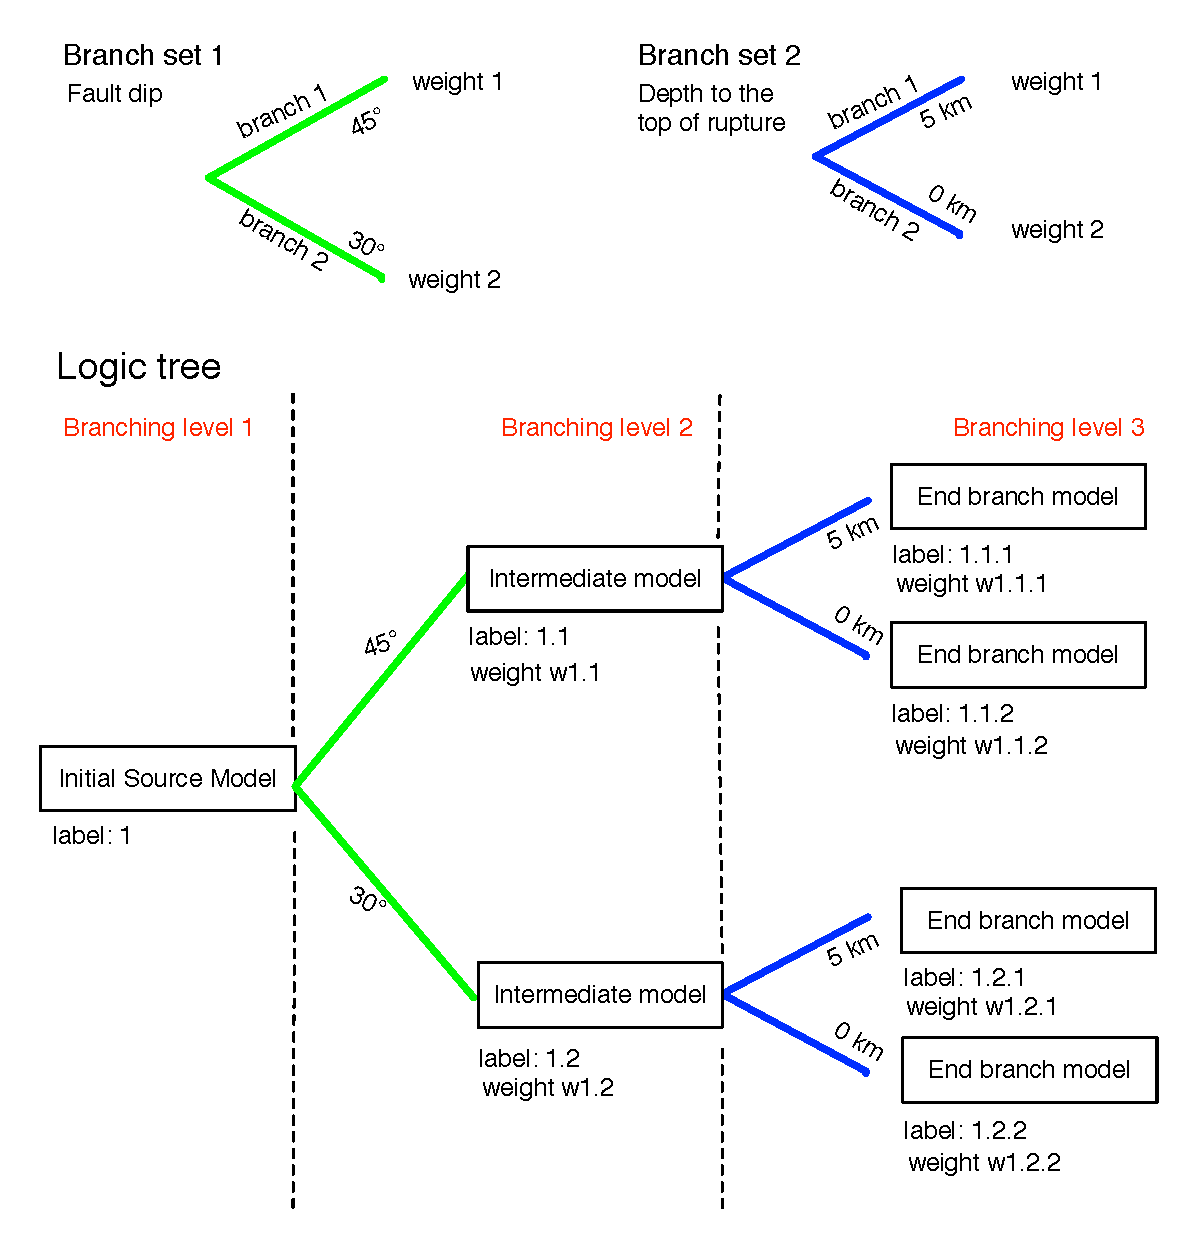
\includegraphics[width=15cm]{./Figures/Part_Hazard/logic_tree_schema.eps}
\caption{Example of a logic tree structure as defined in OpenQuake. The upper
part of the Figure depicts two branching levels.}
\label{fig:logic_tree_schema}
\end{figure}
% . . . . . . . . . . . . . . . . . . . . . . . . . . . . . . . . . . . < Figure
%
We use this logic tree description to specify the structure of the Seismic Source Logic Tree as well as for the Ground Motion Prediction Equation Logic Tree. 

%In the following paragraphs we provide a detailed description of these
%Logic Tree structures.
%%
%%  - - - - - - - - - - - - - - - - - - - - - - - - - - - - - - - - - - - - - - -
%\subsection{Seismic Source Logic Tree description and the Seismic Sources system}
%\index{Seismic Sources System}
%%
%OpenQuake uses a Seismic Source Logic Tree to describe epistemic uncertainties affecting parameters - or elements (e.g. the geometry of an area seismic source) - being part of a Seismic Source Model. 
%%
%%  - - - - - - - - - - - - - - - - - - - - - - - - - - - - - - - - - - - - - - -
%\subsection{Ground Motion Prediction Equation Logic Tree description and the GMPE System}
%%
